\section{Question 5}
In this question we are asked to perform 2-means clustering and report the 21 dimensional centers. Then project the centers onto the plot of the principle components and discuss the results.
\subsection{Description of software}
In addition to the software described in section \ref{q4} I also use the \cite{scikit-learn} implementation of K-Means. The K-means implementation takes the the number of clusters, in our case \(2\), after which it is fit on the data set. The implementation has an attribute \texttt{cluster\_centers\_} allowing us to access the \(2, 21\)-dimensional clusters sought. 
\subsection{Results}
\begin{figure}[h]
\centering
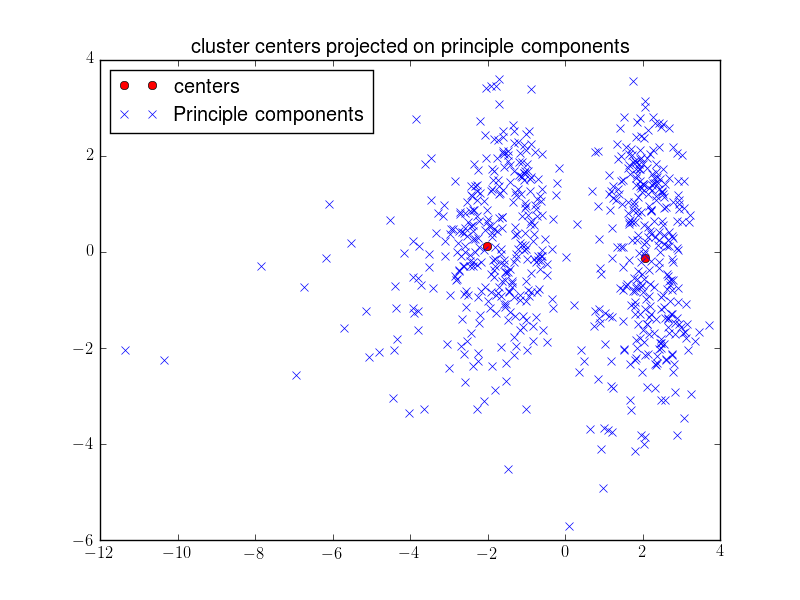
\includegraphics[scale=0.5]{img/clusters.png}
\caption{Clusters}
\label{clusters}
\end{figure}
\newpage
\begin{table}[h]
\centering
\begin{tabular}{ll}
Cluster 1   & Cluster 2   \\\hline
-0.58059034 & 0.59717864  \\
0.31162575  & -0.32052935 \\
0.33137633  & -0.34084423 \\
0.60352028  & -0.62076372 \\
-0.55895616 & 0.57492634  \\
0.39645813  & -0.40778551 \\
0.70939172  & -0.72966006 \\
-0.12401008 & 0.12755322  \\
0.46541403  & -0.47871158 \\
0.23935885  & -0.24619767 \\
-0.06244501 & 0.06422915  \\
0.51736633  & -0.53214823 \\
-0.26469363 & 0.2722563   \\
0.4662318   & -0.4795527  \\
0.03759908  & -0.03867334 \\
0.49394562  & -0.50805835 \\
0.05008879  & -0.0515199  \\
0.53750762  & -0.55286498 \\
-0.27000487 & 0.2777193   \\
0.72935266  & -0.75019131 \\
0.53275234  & -0.54797384\\\hline
\end{tabular}
\caption{K-means centroids}
\label{tab:centroids}
\end{table}

\subsection{Discussion}
The clusters are a projected onto the 2-dimensional plot of the principle components. From the plot we see both centroid nodes are roughly placed in the middle of the principle component space. This suggests that our method of implementing PCA is correct and that the data set does indeed form around the clusters, thus validating the correctness of the components.
